\documentclass[12pt]{article}
\usepackage{fullpage}
\usepackage{multicol}
\usepackage{graphicx}
\usepackage{fontspec}
\usepackage{graphicx}
\usepackage{setspace}
\doublespacing
\setmainfont{OpenDyslexicAlta}
\newcommand{\blk}{\underline{\hspace{0.5in}}}
\begin{document}
%\maketitle
\center{\section*{Geometry Test 2}}
\center{\section*{Work in your notebook.  Show all work for credit!}}
%\begin{multicols}{2}
\begin{enumerate}
\item Calculate: $\displaystyle \sqrt{49}$

\item Calculate: $\displaystyle \sqrt{6^2 + 8^2}$

\item Calculate: $ \sqrt{0.81}$

\item In the right triangle shown below $a=12$, $b=5$, solve for $c$:

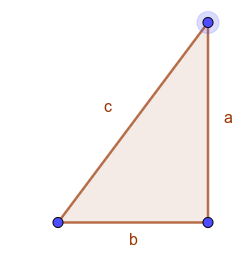
\includegraphics[width=2in]{345triangle.png}

\item In the right triangle shown below $b=6$, $c=10$, solve for $a$:

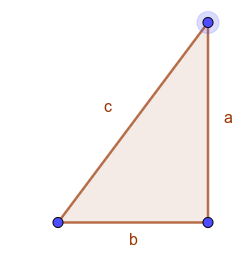
\includegraphics[width=2in]{345triangle.png}

\item Is a triangle with sides $1, \sqrt{2}, \sqrt{3}$ a right triangle?

\item Find the area of the \textbf{shaded} triangle shown below:

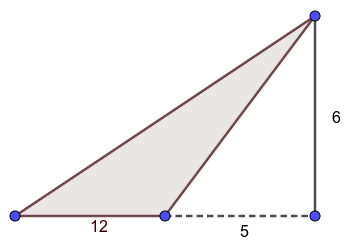
\includegraphics[width=3in]{area-triangle-1.png}

\item Plot the points $A=(-1, 3)$ and $B=(2, 7)$ and calculate the distance between them.

\item Duplicate the angle shown below in your notebook \textbf{only using a straight edge and a compass}.  You may not use a protractor!  Describe how you did it.

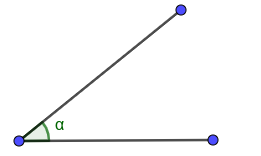
\includegraphics[width=2.5in]{angle-1.png}

\item Find the equation of the line between the points $(2, 1)$ and $(4, 7)$, and sketch the graph.

\pagebreak
\item In the triangle below, find the missing angle without using a protractor.

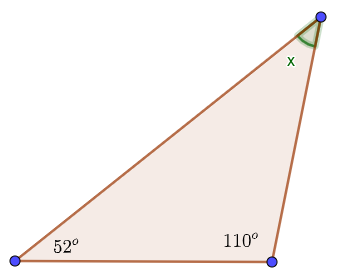
\includegraphics[width=2.5in]{triangle-solve-angle-1.png}

\item In the diagram below solve for the angles $x$ and $y$.  Do not use a protractor.

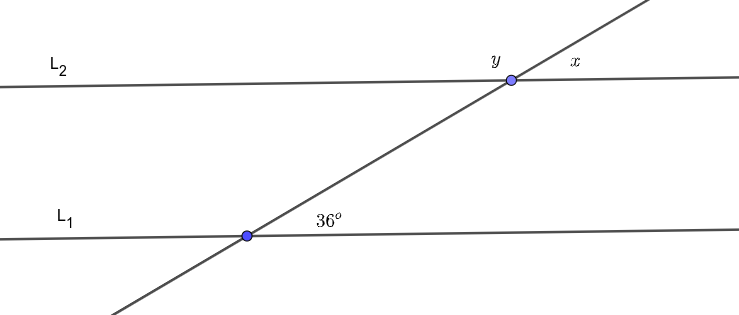
\includegraphics[width=5.5in]{parallel-find-angle-1.png}
\item (Extra Credit:) Our second Pythagorean Theorem proof relied on using 4 copies of the triangle to make a large square with a small square in the center.
\begin{enumerate}
	\item Draw a picture of that.
	\item Use that picture to write an equation calculating the area of the square in 2 different ways.  This is what we did to start our equation in the proof of the Pythagorean Theorem.
	\item Use that equation to prove the Pythagorean Theorem.
\end{enumerate}

\item (Extra Credit) Find the distance between the points $A=(1, 2, 3)$ and $B=(4, 0, 1)$.

%\item (Extra Credit) Find $k$ so that the distance between $(8, 2)$ and $(3, k)$ shall be $13$.


\item (Extra Credit): Write a paragraph about your biography mathematician.  Include at least 3 sentences.
\end{enumerate}
%\end{multicols}
\end{document}